\documentclass[12pt]{article}
\usepackage{graphicx}
\usepackage{amsmath}
\usepackage{geometry}
\usepackage{listings}
\usepackage{color}
\usepackage{array}
\usepackage{hyperref}
\usepackage{url}
\usepackage{tikz} \usetikzlibrary{shapes, arrows.meta, positioning}

\geometry{a4paper, margin=1in}

\definecolor{mygreen}{rgb}{0,0.6,0}
\definecolor{mygray}{rgb}{0.5,0.5,0.5}
\definecolor{mymauve}{rgb}{0.58,0,0.82}

\lstset{
	language=C++,
	basicstyle=\ttfamily\small,
	numbers=left,
	numberstyle=\tiny,
	stepnumber=1,
	numbersep=10pt,
	tabsize=4,
	breaklines=true,
	captionpos=b,
	keywordstyle=\color{blue}\bfseries,
	commentstyle=\color{mygray},
	stringstyle=\color{red}
}

\begin{document}
	\begin{titlepage}
		\centering
		
		\includegraphics[width=0.4\textwidth]{Resources/logo_utcn.png}\\
		\vspace*{6cm}
		
		\Huge
		\textbf{Rendering a Minecraft Scene}
		
		\vspace{0.5cm}
		\Large
		Project Documentation
		
		\vspace{1.5cm}
		
		\textbf{Grad Laurentiu-Calin}\\
		\text{Group 30435}
		
		\vfill
		
		\Large
		Computer Science\\
		January, 2025\\
		
	\end{titlepage}
	
	\newpage
	
	\tableofcontents
	
	\newpage
	
	\section{Subject Specification}
	
	
	
	\section{Scenario}
	\subsection{Scene \& Object Description}
	
	Imagine a serene forest clearing at dusk. In the center stands a tall, weathered watchtower, its silhouette stark against the fading light. Nearby, a majestic tiger prowls silently, its eyes gleaming with a predatory focus. Scattered around the clearing are several tree stumps, remnants of once-mighty trees, now serving as perches for curious deer that cautiously graze the underbrush.
	
	Parked to one side is an old, slightly rusted van, its paint chipped and faded, hinting at many adventures past. Above, the sky is a canvas of twilight hues, and cutting through the clouds are several airships from Star Wars, their sleek, futuristic designs contrasting sharply with the natural beauty below. The hum of their engines adds a surreal, almost otherworldly ambiance to the scene.
	
	It's a place where the wild and the fantastical coexist, creating a unique and captivating tableau.  

	\subsection{Functionalities \& User Manual}
	
	\begin{enumerate}

		\item \textbf{camera movement} - any place in the scene can be reached by moving the camera accordingly; 

		\begin{itemize}
			\item \textbf{W} - move forward
			\item \textbf{A} - move left
			\item \textbf{S} - move backward
			\item \textbf{D} - move right
			\item \textbf{mouse/touchpad} - rotate the camera around all axis
		\end{itemize}

		\item \textbf{automated tour of the scene} - press \textit{T} to start an automated tour of the scene; during this process no input from outside (i.e. mouse, keyboard) is taken into account.		

		\item \textbf{toggle lighting} - press \textit{L} to toggle the flashlight
		\item \textbf{switch between rendering options} - press \textit{1, 2 or 3} to toggle between point rendering, line rendering and polygon rendering
		\item \textbf{change the skybox} - press \textit{N} to swap between skyboxes
		\item \textbf{create a lighning} - press \textit{F} to create a lightning effect
		\item \textbf{bright up the scene more} - press \textit{ARROW UP} to make the scene brighter
		\item \textbf{darken the scene more} - press \textit{ARROW DOWN} to make the scene darker
		\item \textbf{exit} - press \textit{ESC} to exit
		
	\end{enumerate}
	
	\section{Implementation Details}
	
	\subsection{Implementing Directional Shadow Mapping in OpenGL}
	Directional shadow mapping in OpenGL involves creating a depth map from the perspective of a directional light source, such as the sun. This process includes rendering the scene from the light's viewpoint to capture depth information, which is then used to determine shadowed areas during the final rendering pass. Key steps include setting up a framebuffer for the depth map, configuring the light's orthographic projection matrix, and applying a shadow bias to prevent artifacts. The depth map is sampled in the fragment shader to compare the current fragment's depth with the stored depth, allowing for realistic shadow casting and enhancing the scene's depth and realism.

	\subsection{Implementing Omnidirectional Shadow Mapping in OpenGL}
	Omnidirectional shadow mapping in OpenGL is used for point light sources that emit light in all directions, such as a light bulb. This technique requires creating a cubemap to store depth information for six different directions (positive and negative X, Y, and Z axes). The scene is rendered six times from the light's position, each time capturing depth data for one face of the cubemap. In the fragment shader, the depth of each fragment is compared to the corresponding depth value in the cubemap to determine if it is in shadow. This approach allows for accurate shadow casting from point lights, adding a layer of realism to dynamic lighting scenarios.

	\subsection{Implementing a Skybox in OpenGL}
	Implementing a skybox in OpenGL involves creating a seamless 360-degree background that surrounds the entire scene, giving the illusion of a distant environment. This is achieved by mapping six images (or a single cubemap texture) onto the faces of a large cube centered around the camera. The skybox is rendered first, with depth testing disabled, to ensure it appears behind all other objects. The vertex and fragment shaders are used to correctly map the textures onto the cube faces, creating a continuous and immersive background. This technique enhances the visual appeal of the scene by providing a realistic and dynamic sky.

	\subsection{Implementing Point Lights in OpenGL}
	Point lights in OpenGL simulate light sources that emit light equally in all directions from a single point, such as a light bulb. To implement point lights, you need to define the light's position, color, and attenuation factors. The attenuation factors determine how the light intensity decreases over distance. In the fragment shader, the light's contribution to each fragment is calculated based on the distance between the light source and the fragment, as well as the angle of incidence. The Phong lighting model is typically used to compute the ambient, diffuse, and specular components of the light, resulting in realistic illumination and shading effects. This technique is essential for creating dynamic and immersive lighting in 3D scenes.
	

	\subsection{Implementing Spot Lights in OpenGL}
	Spotlights in OpenGL are implemented by defining a light source with a specific position, direction, and cone angle, creating a focused beam of light. The spotlight's properties, such as cutoff angles and attenuation factors, are passed to the shaders. In the fragment shader, the angle between the light direction and the vector from the light to the fragment is calculated to determine if the fragment is within the spotlight's cone. If it is, the light's intensity is computed based on the distance and angle, applying the Phong lighting model to achieve realistic illumination and shadows. This technique is useful for creating dramatic lighting effects and highlighting specific areas in a scene.

	
	\subsection{Functions \& Algorithms}
	
	\subsubsection{Percentage Closer Filtering (PCF) in Shadow Mapping}
	Percentage Closer Filtering (PCF) is a technique used to smooth out the hard edges of shadows produced by shadow mapping. In traditional shadow mapping, shadows can appear jagged and aliased due to the discrete nature of the depth map. PCF addresses this by sampling multiple points around the current pixel in the shadow map and averaging the results. This creates a softer transition between shadowed and lit areas, resulting in more natural-looking shadows. The process involves comparing the depth of each sample point to the depth map and averaging the results to determine the shadow intensity. This technique is widely used in real-time rendering to enhance the visual quality of shadows.
	
	\subsubsection{PCF in Omnidirectional Shadow Mapping}
	Percentage Closer Filtering (PCF) is a technique used to smooth out the hard edges of shadows produced by shadow mapping. In omnidirectional shadow mapping, this technique is particularly useful for point light sources that emit light in all directions. The process involves creating a depth cubemap, which stores depth information for six different directions (positive and negative X, Y, and Z axes). The scene is rendered six times from the light's position, each time capturing depth data for one face of the cubemap.
	
	PCF enhances the shadow quality by sampling multiple points around the current pixel in the shadow map and averaging the results. This creates a softer transition between shadowed and lit areas, resulting in more natural-looking shadows. The depth of each sample point is compared to the depth map, and the results are averaged to determine the shadow intensity. This technique helps to mitigate aliasing and jagged shadow edges, providing a more realistic and visually appealing shadow effect.
	
	In the context of Learn OpenGL, PCF is implemented by sampling the depth cubemap with a direction vector to obtain the closest depth at each fragment. The fragment shader compares the depth of each fragment with the stored depth value in the cubemap to determine if it is in shadow. By averaging the results of multiple samples, PCF produces smoother and more natural shadows, enhancing the overall visual quality of the scene.
	
	\subsection{Graphics Model}
	The project leverages OpenGL 3.3 Core features to achieve high-performance rendering, complemented by GLFW for cross-platform window management and real-time user input handling. GLEW is utilized for the loading of OpenGL extensions where applicable, and GLM serves as the mathematical backbone for vector and matrix transformations.
	
	For content creation, Blender was used to design and assemble assets such as the terrain, military vehicles, and environment props. Each asset underwent preprocessing, including applying accurate scaling, orientation adjustments, and UV unwrapping for optimal texture mapping before export. Textures, sourced ones, were applied to the models.
	
	On top of that, we can mention:
	
	\begin{itemize}
	\item  Shaders: Custom GLSL shaders are used for advanced rendering techniques, including directional and point lighting, shadow mapping, and fog effects.
	\item  Skybox: A procedural or high-resolution image-based skybox frames the environment, contributing to the sense of depth and atmospheric immersion.
	\item  Efficient Asset Integration: Assets were exported in formats optimized for OpenGL (e.g., OBJ), ensuring compatibility while retaining high polygon fidelity for detailed visuals.
	\end{itemize}
	
	This comprehensive approach blends state-of-the-art tools, custom algorithms, and a robust rendering pipeline to deliver a visually compelling and technically sophisticated graphics model.
	
	\subsection{Data Structures}
	The project required several key data structures to manage and render the complex scene efficiently. Camera matrices were essential for handling the camera's position, orientation, and movement, allowing for smooth navigation and dynamic viewpoints. Light properties, including positions, colors, and attenuation factors, were stored in arrays to facilitate the use of multiple light sources and their interactions with objects in the scene. Texture samplers were used to manage and apply various textures to the models, ensuring accurate and detailed visual representation. Additionally, transformation matrices were crucial for positioning, scaling, and rotating objects within the scene. These data structures, combined with efficient algorithms, enabled the creation of a rich and immersive visual experience, seamlessly integrating lighting, shadowing, and environmental effects.
	
	
	\subsection{Class Hierarchy}

	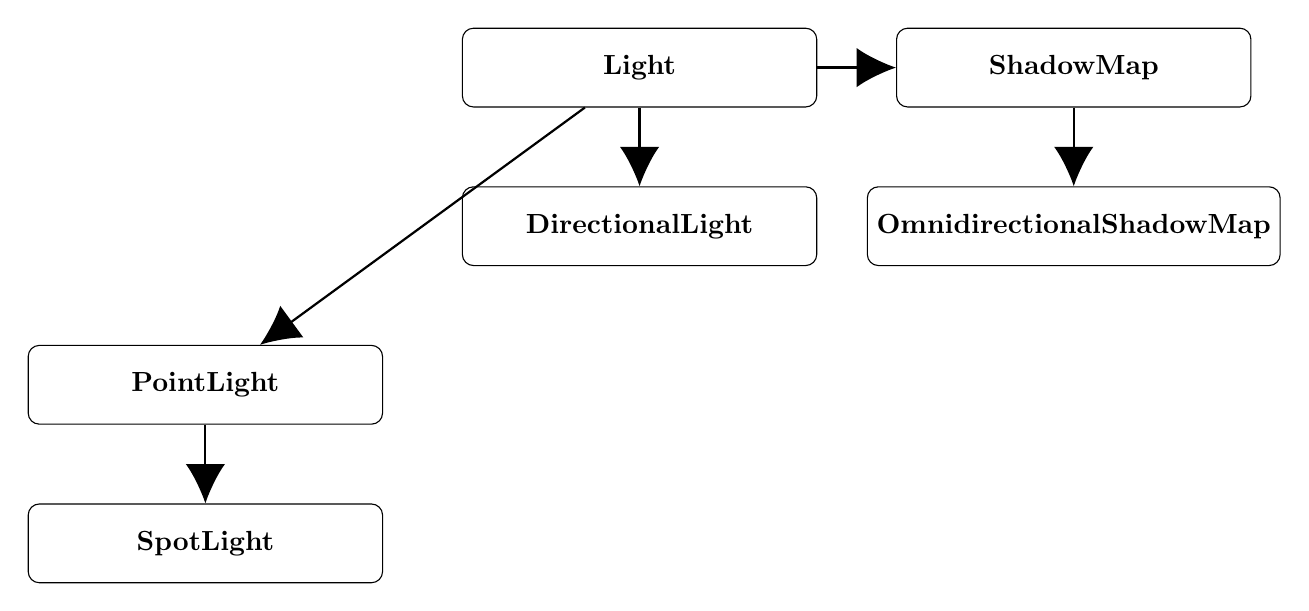
\begin{tikzpicture}[
		class/.style = {rectangle, draw, rounded corners, minimum width=4.5cm, minimum height=1cm, font=\bfseries},
		arrow/.style = {draw, -{Latex[length=5mm, width=5mm]}, thick}
		]
		
		% Classes
		\node[class] (Light) {Light};
		\node[class, below=of Light] (DirectionalLight) {DirectionalLight};
		\node[class, below left=of DirectionalLight] (PointLight) {PointLight};
		\node[class, below=of PointLight] (SpotLight) {SpotLight};
		\node[class, right=of Light] (ShadowMap) {ShadowMap};
		\node[class, below=of ShadowMap] (OmnidirectionalShadowMap) {OmnidirectionalShadowMap};
		
		% Arrows
		\draw[arrow] (Light) -- (DirectionalLight);
		\draw[arrow] (Light) -- (PointLight);
		\draw[arrow] (PointLight) -- (SpotLight);
		\draw[arrow] (Light) -- (ShadowMap);
		\draw[arrow] (ShadowMap) -- (OmnidirectionalShadowMap);
		
	\end{tikzpicture}	


	\section{Conclusions}
	
	Working on this project has been an arduous journey, filled with countless challenges and setbacks. I had to start over twice from the project core and once from scratch, each time facing new obstacles and frustrations. Despite my best efforts, I am not entirely satisfied with the end result. The project did not meet my initial expectations, and there are several aspects that I believe could be significantly improved. However, I am determined to remake the project, learning from my mistakes and refining my approach. This experience has been a valuable learning opportunity, and I am committed to achieving a better outcome in the future.
	
	
	\subsection{Further Developments}
	The project has laid a solid foundation, but there are several areas for potential improvement and expansion:
	
	\begin{itemize}
		\item \textbf{Collision Detection}: Adding collision detection between the camera and environment objects would prevent clipping through terrain and buildings, enhancing the immersive experience.
		\item \textbf{Complex Weather Transitions}: Gradually transitioning between clear skies and storm conditions, including dynamic cloud coverage and heavier rain, would create a more realistic and dynamic environment.
		\item \textbf{Vehicle Animations}: Implementing path-following logic for tanks or half-tracks to drive through the village would add movement and life to the scene.
		\item \textbf{Advanced Sound Design}: Incorporating additional ambient desert noises, such as wind gusts and occasional gunfire echoes, would enhance the auditory experience.
		\item \textbf{Improved User Interface}: Developing a more intuitive and user-friendly interface for controlling scene elements and effects would improve the overall user experience.
		\item \textbf{Performance Optimization}: Further optimizing the rendering pipeline and data structures to improve performance, especially for larger and more complex scenes.
	\end{itemize}
	
	These enhancements would build upon the existing project, creating a more immersive, realistic, and engaging experience for users.
	
	\subsection{References}
	\begin{itemize}
		\item \textbf{Udemy course}:  \url{https://www.udemy.com/course/graphics-with-modern-opengl/}
		\item \textbf{Stack overflow}
		\item \textbf{OpenGL Reference - OpenGL Wiki}: This wiki provides comprehensive documentation for the OpenGL API, including detailed descriptions of each function and their usage across different versions of OpenGL. Available at: \url{https://www.khronos.org/opengl/wiki/OpenGL_Reference}
		\item \textbf{OpenGL - The Industry Standard for High Performance Graphics}: The official OpenGL website offers a wealth of resources, including documentation, tutorials, and reference pages for various OpenGL versions. Available at: \url{https://www.opengl.org/}
		\item \textbf{OpenGL 4 Reference Pages - Khronos Group}: This page provides reference documentation for OpenGL 4, including detailed descriptions of functions and their parameters. Available at: \url{https://registry.khronos.org/OpenGL-Refpages/gl4/}
	\end{itemize}
	
	
\end{document}
